\chapter{本プロジェクトにおける目的}
第3章では、グループBでの目的や目的達成のための目標、今後の展望を紹介する。\\
到達目標では、今後制作していくゲームの紹介や、作成する地域・歴史に基づいた辞書の詳細を紹介している。
\section{グループBにおける目的の概要}
% 担当:田中龍仁
% 1.3節で述べた課題をより具体的に記述する。成果に対して必ず満たすべき条件を含む
これらの背景は、新聞がどのようなものであるかを知られていないことが原因の一つであると考えられる。そこで、新聞が持っている地域性や時代特有の言葉に触れてもらい、新聞の持つ特性を再確認させることを目的とする。以上の目的を達成するために、The New York Timesの事例から言葉遊びゲームを利用することとした。そのため、グループBでは、新聞ビッグデータを利用した辞書を活用したゲームを制作するゲーム開発班と、新聞ビッグデータを利用した地域的・歴史的に基づいた辞書を作成する機械学習班の2つに分かれて活動する。
\bunseki{田中龍仁}

\section{到達目標}
\subsection{ゲーム開発班での到達目標}
% 担当:田中龍仁
グループBでは、新聞ビッグデータから抽出した辞書を使用したゲームの制作を目標としている。現段階では、前期の活動を通して「ヒットアンドブロー」、「制限付き言葉遊び」、「新聞クロス」、「文字アナグラム」、「8パズル」、「検索ゲーム」、「きっちり文字埋め」、「シルエット~これなんだろな~」、「センテンスパズル」の計9個のゲームの制作案が出た。
\begin{itemize}
    \item 「ヒットアンドブロー」では、作成した辞書から抽出した言葉を少ない手数で当てるゲームである。文字が入力されると、HIT(文字も場所も正解)の数と、BLOW(文字は正解だが場所が違う)の数が回答される。それをヒントに正解の言葉を当てるゲームを制作する。
\begin{figure}[htbp]
    \centering
    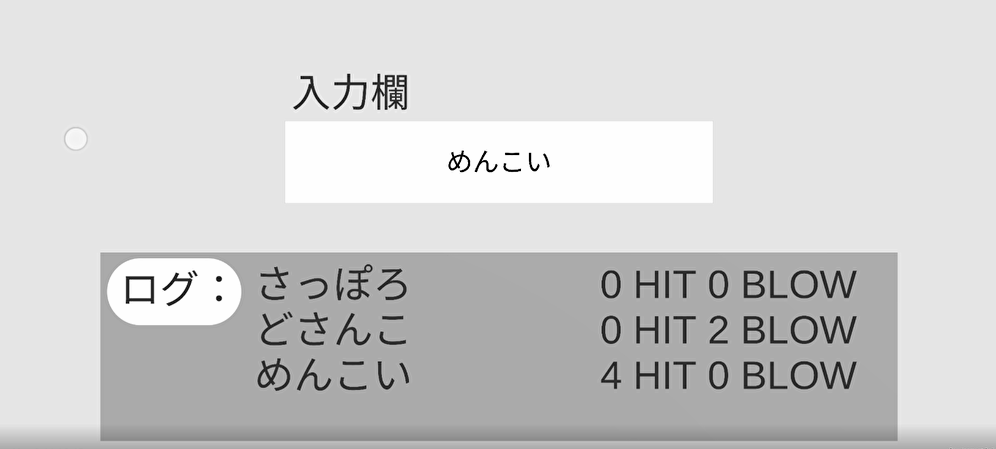
\includegraphics[keepaspectratio, scale=0.3]{images/Project_picuture2.png}
    \caption{「ヒットアンドブロー」の画面}
    \label{fig:my_label}
\end{figure}
\newpage
    \item 「制限付き言葉遊び」では、同じひらがなを2回以上は使えないルールに加えて、さらに時代やお題によって制限された言葉を交互に答え合うゲームを制作する。例えば、50 年前でお題を「北海道の地名」とした場合、「あさひかわ」や「ねむろ」は答えることができる。しかし、「ほくと」を答えてしまうと、北斗市が設置されたのは 2006 年のため使用できない。また、「あさひかわ」と答えた後に次のターンで同じプレイヤが「さっぽろ」を選んでしまうと、「さ」を使用した後にもう一度「さ」を使用しているため、負けとなる。
\begin{figure}[htbp]
    \centering
    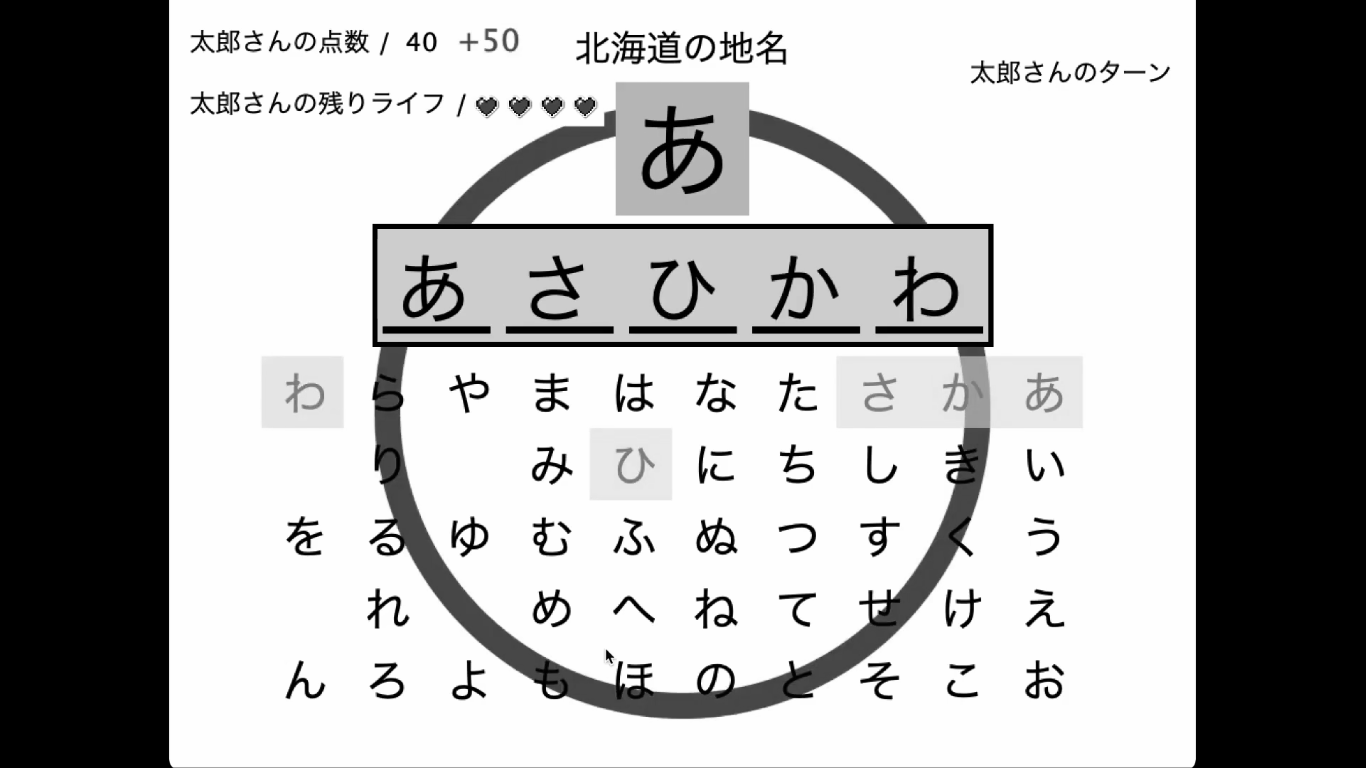
\includegraphics[keepaspectratio, scale=0.2]{images/Project_picuture1.png}
    \caption{「制限付き言葉遊び」の画面}
    \label{fig:my_label}
\end{figure}

    \item 「新聞クロス」では、通常のクロスワードパズルと違い、使われている言葉が北海道に関連したもので作られている。ヒントをもとに、縦・横の文字数に合う言葉を埋めていき、盤面を完成させるゲームを制作する。
\begin{figure}[htbp]
    \centering
    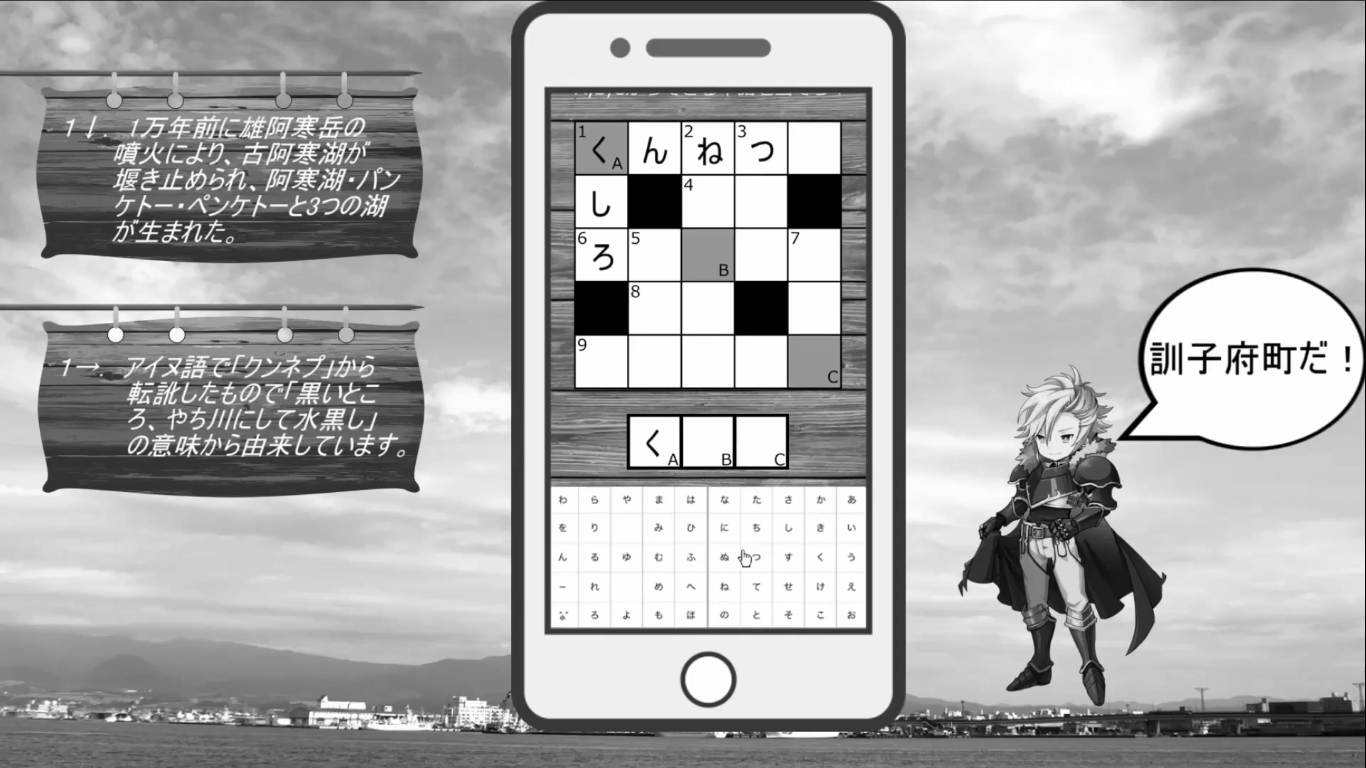
\includegraphics[keepaspectratio, scale=0.2]{images/Project_picuture3.png}
    \caption{「新聞クロス」の画面}
    \label{fig:my_label}
\end{figure}
    \item 「文字アナグラム」では、辞書から抽出した言葉を出題し、出題された言葉をいくつか入れ替えることによって、全く別の意味に変換させるゲームである。例えば、「こさどん」という問題が出題されたとき、文字を入れ替えることで、「どさんこ」という言葉に並び替えることでクリアとなる。\\
    
    \item 「8パズル」では、3×3マスの盤面が用意され、そこには文字の書かれた8つのブロックがある。空白の1マスを利用することで、決められた回数だけブロックを動かしていき最終的により多くの言葉を作るゲームを制作する。\\
    
    \item 「検索ゲーム」では、作成した辞書から北海道に関連した言葉をランダムに抽出し、その言葉がいつの年代の記事に一番現れたかを2人のプレイヤがそれぞれ予想する。予想した年代が一致、もしくは近いプレイヤが勝者となるクイズ形式のゲームを制作する。\\
    
    \item 「きっちり文字埋め」では、新聞の型に収まるように、2人のプレイヤが交互に文字を埋めていく。2人のプレイヤが交互に50音から 1 文字を選び、北海道に関連した言葉を作っていく。決められた手数で多くの言葉を作ることのできたプレイヤが勝利するゲームを制作する。\\
    
    \item 「シルエット~これなんだろな~」では、北海道に関連したシルエットを出題し、そのシルエットが何を表しているか当てるゲームを制作する。例えば、「メロン」のシルエットを出題されたプレイヤはそのシルエットが何を表しているかを予想し、解答する。プレイヤが「メロン」と答えることができたらクリアとなる。\\
    
    \item 「センテンスパズル」では、分解された新聞記事を完成させるために、プレイヤがフィールド上方からランダムに1種類ずつ落下してくる。文字が書かれた片面型テトロミノ状のブロックピースを上手く組み合わせて記事を完成させることで、クリアとなる。\\
    
\end{itemize}
\bunseki{田中龍仁}


\subsection{機械学習班での到達目標}
% 担当:保土沢朋和
新聞ビッグデータを利用した地域・歴史に基づいた辞書の作成を目標としている。地域的側面では北海道に関連した言葉をまとめ、歴史的側面では、それぞれの時代によって使われてきた言葉をまとめる。地域的側面の例としては、「函館」、「長万部」といった北海道の地名や「しゃっこい」、「したっけ」といった方言など、北海道でよく使われる言葉を辞書としてまとめる。歴史的側面の例として、「五稜郭タワー」は 1964 年に建造されたため、それより以前の時代では新聞に「五稜郭タワー」という言葉は存在しない可能性がある。このような、特定の時代には使われているが、それ以前やそれ以降には使われていなかった言葉などを辞書としてまとめる。また、年代ごとに、出現回数の多い言葉や特定の地域ではよく使われている言葉などをまとめることで、ゲーム開発班に提供できるような辞書を作成する。これらのような辞書を作成するために、自然言語処理を用いて開発を行う予定である。
\bunseki{保土沢朋和}

\newpage
\section{今後の展望}
\subsection{ゲーム開発班での開発手段・課題}
% 担当:田中龍仁
ゲーム開発班では、ゲームを開発するにあたってUnityというゲームエンジンを利用する。そこで、Unityを使用するための知識とスクリプトを書く際に使用されるC\#言語の知識の習得が必要である。

\bunseki{田中龍仁}

\subsection{機械学習班での開発手段・課題}
% 担当:保土沢朋和
機械学習班では、新聞ビッグデータを分析するにあたって Pythonを利用する。Pythonとは機械学習の分野で使われるプログラミング言語である。その中で、画像の文字をテキストに変換するために文字認識の知識の習得が必要である。さらに、地域や歴史に基づいた辞書を作成するために自然言語処理や機械学習の知識の習得も必要である。
\bunseki{保土沢朋和}

\section{メンバの割り当て}
% 担当:
グループBではゲーム開発班と機械学習班に分けた。ゲーム開発班は主に成果物であるゲームを作成する班であり、機械学習班はゲームを開発するために使われる新聞データを利用した辞書を作る班である。ゲーム開発班には岩上慎之介、田中龍仁、伊藤太一、小山内魁人、中川翔真の5人が割り当てられた。機械学習班には保土沢朋和、日置竜輔、金澤快飛の3人が割り当てられた。
\bunseki{田中龍仁}